\documentclass[12pt]{article}
\usepackage{natbib}
\usepackage{hyperref}
\usepackage{graphicx}
\usepackage{subcaption}
\usepackage{amssymb,amsmath,amsthm}
\usepackage{xcolor}
\usepackage{xspace}
\usepackage[nameinlink,capitalize]{cleveref}
\usepackage{cleveref}
\usepackage{geometry}
\usepackage{pdflscape}

% https://tex.stackexchange.com/questions/12703/how-to-create-fixed-width-table-columns-with-text-raggedright-centered-raggedlef
\usepackage{array}
\newcolumntype{L}[1]{>{\raggedright\let\newline\\\arraybackslash\hspace{0pt}}m{#1}}
\newcolumntype{C}[1]{>{\centering\let\newline\\\arraybackslash\hspace{0pt}}m{#1}}
\newcolumntype{R}[1]{>{\raggedleft\let\newline\\\arraybackslash\hspace{0pt}}m{#1}}

\usepackage{xspace}

\newcommand{\Rlogo}{R\xspace}
\newcommand{\percap}{\emph{per capita}\xspace}
\newcommand{\Rnum}{\mathcal{R}_0}
\newcommand{\comment}{\showcomment}
\newcommand{\showcomment}[3]{\textcolor{#1}{\textbf{[#2: }\textsl{#3}\textbf{]}}}
\newcommand{\nocomment}[3]{}

\newcommand{\fady}[1]{\comment{cyan}{Fady}{#1}}
\newcommand{\ali}[1]{\comment{magenta}{Ali}{#1}}
\newcommand{\jd}[1]{\comment{blue}{JD}{#1}}
\newcommand{\djde}[1]{\comment{red}{DJDE}{#1}}
\newcommand{\bmb}[1]{\comment{red}{BMB}{#1}}
\newcommand{\todo}[1]{\comment{red}{TODO}{#1}}

\theoremstyle{definition} % amsthm only
\newtheorem{proposition}{Proposition}
\newtheorem{theorem}{Theorem}

\bibliographystyle{apalike}

\title{Testing and Isolation Efficacy; Insights from a Simple Epidemic Model }

\begin{document}
\maketitle

% %%%%%%%
\section{Abstract}

% %%%%%%%
\section{Introduction}

The observed dynamics of the COVID-19 epidemic are driven by both epidemiological processes (infection and recovery) and testing processes (testing and test reporting). In addition to shaping epidemic observations (via case reports), testing processes can also affect epidemiological dynamics. In particular, individuals who are awaiting the results of a test may partially or fully self-isolate, and individuals who have tested positive are highly likely to self-isolate. We developed a model that incorporates mechanistic epidemic processes and testing in order to explore the effects of testing and isolation on epidemic dynamics.

Because individuals who have been tested or received a positive test are likely to self-isolate, thus reducing or eliminating  their potentially infectious contacts, the dynamics of an epidemic will depend on who gets tested and
why. For a given testing intensity (tests performed per day), testing will have a stronger effect on infection rates
the more strongly it is focused on people who are infectious for SARS-CoV-2.
This level of focus depends in turn on the purpose and design of testing programs.
(1) When testing is done for the purposes of disease surveillance \citep{foddai2020base}
we might expect tests to be assigned randomly across the population (in an ideal world: some bias in selection for testing is probably inevitable), although a stratified sampling design would be preferred for statistical efficiency \citep{graubard1996modelling} \ali{better ref?}.

Over the course of the COVID19 \ali{consistency COVID-19 or COVID19?} pandemic, however, the vast majority of testing has been done with other goals --
primarily diagnosis (determining COVID19 infection status for clinical purposes), or control (determining COVID19 status in order to quickly isolate cases that have been found by contact tracing), which we characterize as \emph{targeted} testing strategies.
In these cases, testing probabilities vary widely across epidemiological compartments; in our dynamical model, we will characterize these probabilities by assigning a \percap testing weight to each compartment that determines the \emph{relative} probability that an individual in that compartment will be selected for testing (see Methods). 

When testing is used primarily for diagnosis it will focus on people with COVID19-like symptoms; thus the testing weights for people with vs. without SARS-CoV-2 infections will depend on the relative magnitudes of the probability of having COVID19-like symptoms when infected with SARS-CoV-2 (i.e. the relative proportions of presymptomatic or asymptomatic vs. symptomatic infections) and the probability of having COVID19-like symptoms when \emph{not} infected (e.g. due to other respiratory illnesses). Testing for epidemic control will focus on people who are known to have been in contact with known COVID19 cases; in this case the testing weights for infected vs. uninfected people will depend on the probability of infection given contact, as well as the thoroughness and effectiveness of the system for identifying suspicious contacts.

In addition to the overall testing intensity, the testing weights for different compartments, and the degree of self-isolation of test-pending and test-confirmed people, our models will also need to include test specificity and sensitivity, as well as the distribution of times from testing to reporting. 
Here, we focus on the the effect of testing intensity, different levels of testing ``focus'' (from random to highly targeted), and rate of test processing on a single index of epidemiological dynamics, the basic reproduction number $\Rnum$.

The early dynamics of an epidemic are determined by $\Rnum$. This index is defined as the expected number of secondary infections arising from a typical infective individual in a completely susceptible population \citep{dietz1993estimation}. 
In the early stages of an epidemic the number of infected individuals is expected grow exponentially over time when $\Rnum>1$. 
To control the spread of disease in the population, $\Rnum$ must be $<1$.
Although the value of $\Rnum$ cannot completely characterize the dynamics of even the simplest epidemic model
\citep{shaw2021what}, it does give a simple and widely accepted index for the difficulty of control, as well as some indication of the likely final size of an epidemic \citep{ma2006generality}.

% %%%%%%%
\section{Methods}

We developed a deterministic model, Eqs. \eqref{model}, which groups individuals based on disease status and testing status. Disease states include Susceptible, Infectious and Recovered (thus this is an SIR-type model), and testing status categorizes people as \emph{untested}, waiting-for-\emph{positive}, waiting-for-\emph{negative}, or \emph{confirmed positive} (Figure~\ref{fig:flowchart}). Two `accumulator' compartments, $N$ and $P$, were also incorporated in the model in order to collect cumulative reported negative or positive tests. The model and details of calculation of $\Rnum$ are presented in the Supplementary Materials.

\begin{figure}[!h] 
\begin{center} 
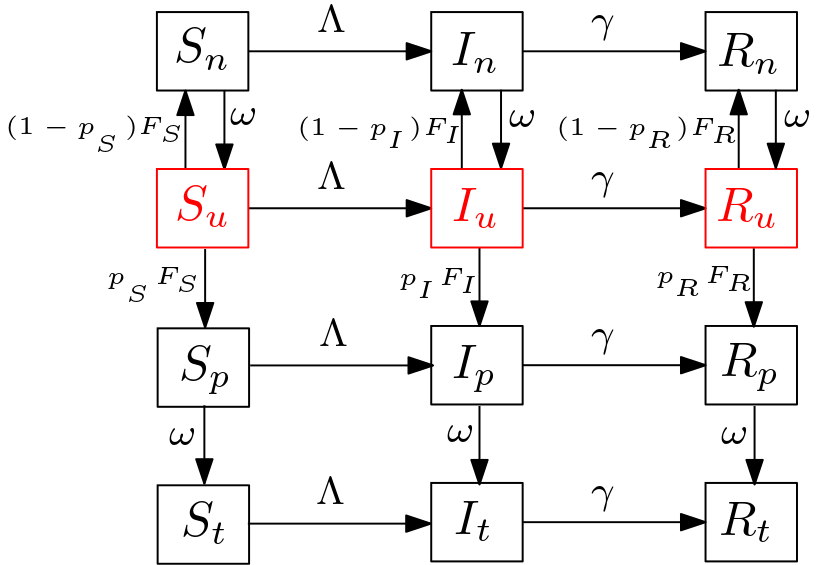
\includegraphics[scale=0.3]{./pix/sir_comp.png}
\caption{\small Flowchart of the SIR (Susceptible-Infectious-Recovered) model, \ref{model}. For the description of the parameters see \cref{tab:params}.
\label{fig:flowchart}}
\end{center} 
\end{figure}

Table~\ref{tab:params} defines the model parameters, which are generally straightforward
\percap flows between compartments, or modifiers to these flow rates.
The novel component of the model comes in through the compartment-specific relative testing weights $W_S$, $W_I$ and $W_R$; these give the relative rates at which people in the $S$, $I$, and $R$ compartments are tested, respectively. For example, $W_I/W_S=2$ means that infected individuals are tested at twice the \percap rate of susceptible individuals. 

In order to link to more applied models, we constructed this model so we could specify the total \percap testing rate. We do this by defining the weighted size of the testing pool $W = W_S S_u + W_I I_u + W_R R_u$, and calculating the scaling parameter for testing as:
\begin{equation}
\label{sigma}
\sigma = \frac{\rho N_0}{W}.
\end{equation}
Thus, \percap testing rate for compartment $Z$ is $F_Z=\sigma W_Z$, where $Z \in \{S,I,R\}$.
For a high-sensitivity test, infected people typically flow through to the ``confirmed positive'' ($I_c$/$R_c$) compartments and are thus unavailable for further testing.
Over the course of the epidemic, a fixed testing rate as specified in \eqref{sigma} can
(if large enough) exhaust the pool of people available for testing,
leading to a singularity when no one is left untested.
Although this phenomenon does not affect our analysis of $\Rnum$, it does sometimes occur in
numerical solutions of the time dynamics: we discuss an adjustment to the model that solves
this problem in the Supplementary material. 

The classical SIR model is based on the following implicit assumptions; well-mixed population, homogeneity of the population, exponentially distributed duration of infection and large population size (see, e.g., \cite{keeling2011modeling}). In addition to these standard assumptions, our model, \ref{model}, assumes: (i) there is a single force of infection, $\Lambda$, defined as follows
\begin{equation}
\label{Lambda}
\Lambda=\beta \frac{(I_u+\eta_w I_n+\eta_w I_p+ \eta_c I_c)}{N_0},
\end{equation}
across all susceptible pools (see Table~\ref{tab:params} for detail), (ii) $\eta_c \leq \eta_w$, i.e., the individuals awaiting test results have a higher transmission probability than the reported individuals. For this analysis, we also assume a perfectly specific test,($p_S=0$). This last assumption combined with the assumption that no individual is in waiting-for-\emph{positive} or \emph{confirmed positive} compartments, i.e., $S_p(0)=S_c(0)=0$, reduces the model to 10 equations (equations c and d  in \eqref{model} are eliminated).

\begin{table}[htp]
\centering
\begin{tabular}{|c|L{2in}cc|} \hline
  Symbol & Description & Unit & Value \\ \hline
  $N_0$     & Total population size & people & $10^6$ \\ \hline
  $\omega$  & Rate of onward flow from ``waiting'' to ``confirmed'' or ``untested'' compartments  & 1/day & - \\ \hline
  $\gamma$ & Recovery rate & 1/day & 1/3 \\ \hline 
  $\rho$   & Per capita testing intensity & 1/day & 0.01 \\ \hline 
  $\eta_w$  & Relative probability of transmission for ``waiting'' individuals & - & - \\ \hline
  $\eta_c$  & Relative probability of transmission for ``confirmed positive'' individuals & - & -  \\ \hline
  $\beta$ & Transmission rate & 1/day & 0.39 \\ \hline
  $\Lambda$ & Force of infection & 1/day & - \\ \hline
  $p_S$ & Probability of positive tests for $S$ ($= 1-\textrm{specificity}$) & - & 0 \\ \hline
  $p_I$ & Probability of positive tests for $I$ ($= \textrm{sensitivity}$) & - & 1 \\ \hline
  $p_R$ & Probability of positive tests for $R$ ($= 1-\textrm{specificity}$) & - & 0.5 \\ \hline
  $W_S, W_I, W_R$ & Relative testing weights & - &
  \begin{minipage}[t]{0.21\columnwidth}%
    Random: $\{1,1,1\}$ \\ Targeted: $\{0.3,1,1\}$
  \end{minipage} \\
  \hline
  \end{tabular}
\caption{\label{tab:params} Parameters of the model \eqref{model}.}
\end{table}

The Disease-Free Equilibrium (DFE) for the SIR model, Eqs. \eqref{model}, is given by solving the coupled system including $S_u+S_n=N_0$ and $F_S S_u-\omega S_n=0$. The DFE is

\begin{equation}
\label{dfe}
S_n^*= \frac{\rho}{\omega} N_0, \ S_u^*= N_0-S_n^*, \text{~and~} I_j=R_j=0 \ \text{for all j}.
\end{equation}

The basic reproduction number, $\Rnum$, was calculated by using the next generation matrix method developed by \cite{van2002reproduction}. $\Rnum$ is

\begin{equation}
\label{R0}
\Rnum= (A \times S_u^* + B \times S_n^*) \times C, 
\end{equation}
where
\begin{align*}
A=& \gamma(\omega+\gamma) + (\gamma \eta_w + \omega \eta_c p_I) F_I, \\
B=& \big(\omega+(F_I+\gamma)\eta_w\big) \gamma+\frac{(\eta_w \gamma+ \eta_c\omega) \omega p_I F_I }{\omega+\gamma}, \\ 
C=& \frac{\beta/\gamma}{N_0 (\gamma(\omega+\gamma)+F_I(\gamma+\omega p_I))}.
\end{align*}
Further details of derivation of $\Rnum$ are provided in the Supplementary material section.
 
The analytical calculation of the next generation matrix, $G$, and the derivation of $\Rnum$ was carried out in Maple (ref?) by using simple linear Algebra package. 
  We used R for the simulation part which included using the explicit expression of $\Rnum$ \ref{R0} as a function of the underlying parameters, specifying the parameters a realistic range, calculating the corresponding $\Rnum$ and plotting the contours of $\Rnum$ by using ggplot package in R. The related result is presented in Figure \ref{pan}, where  panel \eqref{p.a} represents the random testing, and panel \eqref{p.b} is representing non-random testing. The parameter values or ranges are as follows (I like using a table here, with the param, their units and values). It is notable that in the simulation part, the explicit expression of $\Rnum$ was used and not the approximation \eqref{eq:R0appr}. This simulation reflects the behavior of $\Rnum$ with respect to the selected parameters for two different testing strategies: (i) random testing, represented by all testing weights to be the same, $W_S=W_I=W_R$, and (ii) non-random testing, when testing weight are not equal. For simulation purposes we chose $W_S=W_I=W_R=1$ for random testing, and $W_S=0.3$ and $W_I=W_R=1$ for non-random testing strategy. Note that the critical contour of $\Rnum=1$ is plotted in solid line in Figure \ref{pan}. 

% %%%%%%%
\section{Results}

The explicit formula for the basic reproduction number, $\Rnum$ \eqref{R0}, provides an opportunity to study the influence of changes in the underlying parameters on the critical index of epidemic dynamics. We are interested in understanding the effect of parameters that can be realistically controlled by changing in isolation, \percap testing intensity and test resulting, i.e., $\eta_c$ and $\eta_w$, $\rho$ and $\omega$, respectively. The following Proposition is the direct result of taking partial derivative of $\Rnum$ \eqref{R0} with respect to selected parameters. Note that we used Taylor approximation of $\Rnum$ at $\rho=0$ due to the complexity of the expression and thus inconclusive. See the Supplementary material for details.

\begin{proposition}
\label{prop1}
Using the expression of $\Rnum$ \eqref{R0},
\begin{enumerate}
\item \label{p1:eta}
$\partial{R_0}/\partial{\eta_c} \geq 0$ and $\partial{R_0}/\partial{\eta_w} \geq 0$. 
\item \label{p1:rho}
$\partial{\Rnum}/\partial{\rho} \leq 0$ when $\rho \approx 0$.
\item \label{p1:omega}
$\partial{R_0}/\partial{\omega}$ can be positive or negative when $\rho \approx 0$.
\end{enumerate}
\end{proposition}

 Given that the perfect isolation occurs at $\eta_c=\eta_w = 0$, Prop.~\ref{p1:eta} means that lifting the isolation from awaiting group results in an increased $\Rnum$ and consequently a greater number of infected individuals. Prop.~\ref{p1:rho} indicates that increasing the \percap testing intensity, $\rho$, reduces $\Rnum$. Lastly, Prop.~\ref{p1:omega} means that speeding up the test reporting may or may not reduce $\Rnum$, it will depend on other parameters. It is straightforward to derive \ref{p1:rho} and \ref{p1:omega} from the Taylor approximation of $\Rnum$ at $\rho=0$. 
 
\begin{figure}[h!]
\centering
\begin{subfigure}[t]{.45\textwidth}
\centering
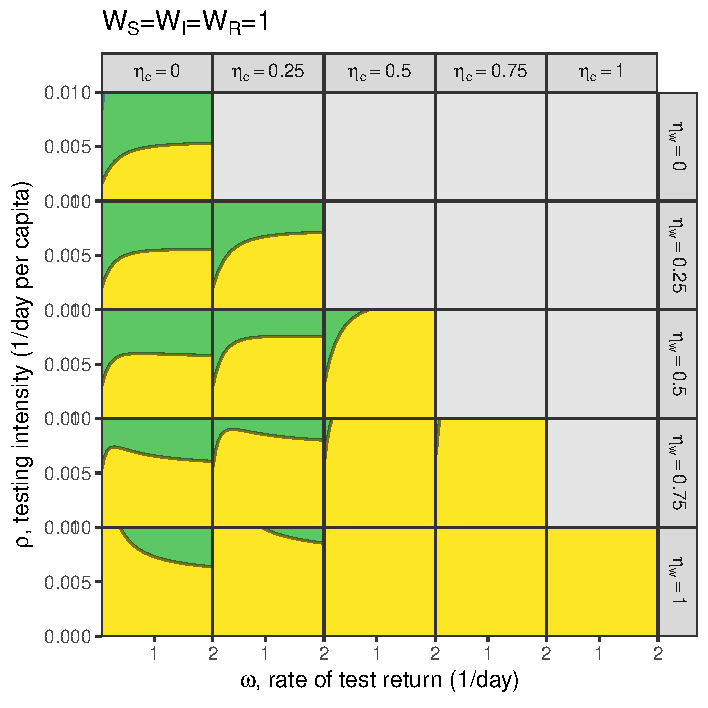
\includegraphics[width=\linewidth]{./pix/R0contour_random.pdf}
\caption{}\label{p.a}
\end{subfigure}
%
\begin{subfigure}[t]{.45\textwidth}
\centering
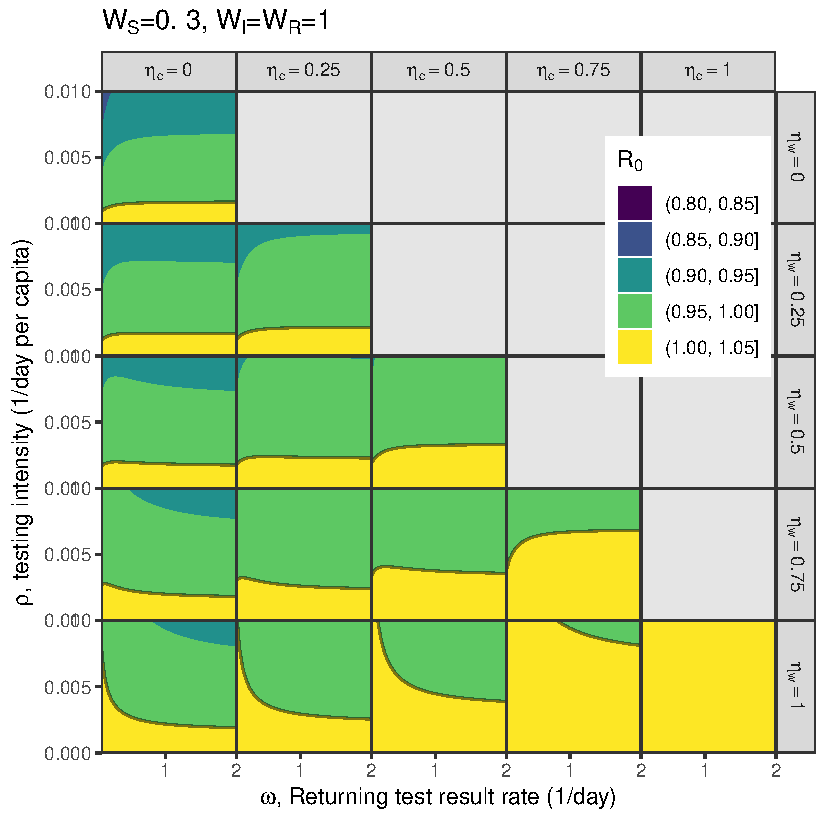
\includegraphics[width=\linewidth]{./pix/R0contour_TTI.pdf}
\caption{}\label{p.b}
\end{subfigure}
\caption{Behaviour of the basic reproduction number, $\Rnum$, with respect to changes in the underlying parameters; \bmb{remind the reader about the parameters and their values}. The solid line in each panel represents the critical contour of $\Rnum=1$. \bmb{we still have some collisions in the y-axis tick labels}}
\label{pan}
\end{figure}

Our numerical solutions in support of the analytical results in Proposition \ref{prop1} are presented in Figure \ref{pan}. It can be inferred that when random testing strategy is applied, Figure \ref{p.a}, comparing to the targeted testing strategy, Figure \ref{p.b}, the critical \percap testing intensity of the corresponding panels are lower in non-random testing. Also, it appears that speeding the test reporting, i.e., increasing $\omega$, does not significantly lower $\Rnum$ when awaiting people (including people in $I_p$ and $I_n$ compartments) follow the isolation perfectly, i.e., $\eta_w$ is closer to 0. However, speeding the test reporting reduces the epidemic more when the awaiting people less follow the isolation, i.e., $\eta_w$ is closer to 1. 

Furthermore, we derived an inequality that quantifies the exact relationships between model parameters that result in returning tests more rapidly being favorable \eqref{eq:necsuf}. 

%%%%%%%%%%%%
\section{Discussion}

Mathematical modeling of infectious disease outbreaks provides insights on how testing processes influence the epidemiological processes through isolation. 
Here, we develop a compartmental SIR-type model to study the potential effect of testing strategies, testing intensity, test sensitivity and specificity, test reporting time and isolation on epidemic dynamics. 
While targeted testing strategies are always more effective than random testing, as expected, we find that in some cases the direct effect of testing is viral spread is expected to be stronger for a slow test than for a fast test. This counter-intuitive effect can occur when people are cautious when awaiting a test result, and may not be robust to second-order effects of fast testing (such as better contact tracing).

We compared two testing strategies, random and \emph{tergeted}, by incorporating the compartment-specific relative testing weights $W_S$, $W_I$ and $W_R$. Although, in this study for the purpose of simplicity and illustraition, we assumed $W_I/W_S=3$ for the targeted strategy scenario, we have not specified a particular relative testing weights corresponding to a particular targeted testing scenario. 
Modeling different targeted testing strategies, thus test-specific testing weights, requires prior information of the conditional probabilities of getting tested for people in a given compartment. This part needs to be developed further in future work. 
This can be implied when we would like to quantify and compare the effect of different levels of test forcus for infectious people on the basic reproduction number $\Rnum$, and conclude about the disease spread management. For example, when people are tested for "screening", the individuals with potential higher mobility, eg. people who are getting on flights, get more tested and thus the coresponding heavier testing weight is assigned than people awaiting for a surgery and are probably going to stay in a long-term care facility and consequently less mobile and more isolated to begin with. With our model, we would be able to compare the sensitivity of the disease dynamics, through $\Rnum$, with respect to testing processes.

{\bf \percap testing intensity, $\rho$};
Proposition \ref{prop1} part \ref{p1:rho} indicates that increasing testing intensity $\rho$ reduces $\Rnum$. This is sensible since as people are moved to test compartments, namely $I_p$ and $I_n$ in particular, may partially or fully self-isolate, and individuals who have tested positive, namely $I_c$ compartment, are highly likely to self-isolate. The higher probability of being subject to isolation, the lower the transmission \eqref{Lambda} will become and the lower $\Rnum$ will become. Our simulation supports this fact. However, it appeared to be hard to conclude this by directly differentiating the expression of $\Rnum$ due to its complexity.  

{\bf Delay in test reporting rate, $\omega$};
Proposition \ref{prop1} part \ref{p1:omega} is the most interesting result. It states that returning test results more rapidly, i.e., increasing $\omega$, does not necessarily lower $\Rnum$; whether increasing $\omega$ lowers $\Rnum$ depends on the precise combination of model parameters (test reporting rate, testing processes/strategies ($W_*$), testing efficacy ($P_I$) and isolation ($\eta_*$). Specifically, the $\partial{R_0}/\partial{\omega}>0$ suggests that reproduction number may increase as the test reporting process become faster. This can be seen from expression \eqref{Rom} in the case of perfect isolation, when $\eta_w=0$ and $\eta_c=0$. The underlying mechanism for this result is that individuals may take more precautionary behaviors (e.g., physical distancing) when they are awaiting test results compared to when they are untested or their test has returned negative. An example of a situation that would favour slow return of tests is if the test being employed produces many false negatives, because many infected individuals will believe they are negative and thus may unknowingly spread the virus to many others.  For an example of the behaviour of $\Rnum$ see Figure \ref{pan} at varying values of $\omega$. This property also provides a tool to quantify the amount of delay required in the test reporting process as a strategy to reduce $\Rnum$ and consequently control the epidemic.   


To give a biological interpretation, we describe the qualitative trends predicted by the inequality. Returning test results more rapidly tends to be more favorable, i.e., reduces $\Rnum$, when (i) \emph{Confirmed-positive} individuals, lower their contact much more than individuals who are waiting for their test results (i.e., $\eta_c \ll \eta_w$), (ii) the test is highly sensitive, i.e., $p_I$ is close to 1, and (iii) the targeted testing strategy is practiced. An in-depth discussion of these results is presented in the discussion section. 

- The use of tests cheaper than RT-PCR has been proposed as a potential strategy for containing the COVID-19 pandemic. While cheaper tests may be less sensitive and reliable than RT-PCR, they allow for broader and more intense testing. Using our Taylor approximation of $\Rnum$ near $\rho = 0$, we examined what circumstances (i.e., model parameters) make the use of one test more favourable than another, and give a complete description through inequality \ref{eq:rho1vsrho2}. In general, we found that the expensive test tends to more effectively lower $\Rnum$ when (a) individuals who test positive self-isolate much more than individuals who are waiting for their test result, (b) the time it takes to return tests is much shorter than the mean infectious period, and (c) the testing intensity is much greater for infected individuals than susceptible individuals.
- Our model also predicts an asymmetry between cheap and expensive tests: if a cheap test can identify on average more infected individuals as an expensive test, then our model predicts that the cheap test will lower $\Rnum$ more. In contrast, if an expensive test can identify on average more infected individuals, it will not necessarily lower $\Rnum$ more than the cheap test. 

{\bf Other points};
one point we can make when discussing the relative weight of testing in different compartments is to discuss pre-testing screening tools, such as surveys or questionnaires. If we have a quantitative description of how the testing intensities affect the dynamics, we can make statements like ``our results suggest that employing a pre-testing screening tool can help target infected individuals more effectively. In particular, doubling the sensitivity of the pre-screening tool would *do something* to $\Rnum$.

% JD:
% \begin{itemize}
%  \item We're basically looking at the potential advantage of slow tests:
% people waiting for test results may be more careful than those who
% have received negatives. These advantages are real, and neglected. We
% also compare to an individual-level advantage of fast tests: people
% who test positive may be even more careful. But we are missing out on
% community-level advantages of fast testing: better assessment of the
% situation, identification of hot spots, contact-tracing, etc. 
% \item  Maybe something about the testing rate/intensity, now the per capita testing intensity is very low ($\rho \approx 0$). In near future new test kits may be widely accessible, our model provide insights in this case (what are those?)
% \item ``delay negative results" result
% \end{itemize}

% %%%%%%%
\bibliography{SIRlibrary}

% %%%%%%%%%%%%%%%%%%%%%%%%%%%%%%%%%%%%%%%%%%%%%%%%%%%%%%%%%%%%%%%%%%
\clearpage
% \widetext
\begin{center}
\textbf{\large Supplemental Materials: Title for main text}
\end{center}
%%%%%%%%%% Merge with supplemental materials %%%%%%%%%%
%%%%%%%%%% Prefix a "S" to all equations, figures, tables and reset the counter %%%%%%%%%%
\setcounter{equation}{0}
\setcounter{figure}{0}
\setcounter{table}{0}
\setcounter{page}{1}
\makeatletter
\renewcommand{\theequation}{S\arabic{equation}}
\renewcommand{\thefigure}{S\arabic{figure}}
\renewcommand{\bibnumfmt}[1]{[S#1]}
\renewcommand{\citenumfont}[1]{S#1}
%%%%%%%%%% Prefix a "S" to all equations, figures, tables and reset the counter %%%%%%%%%%

\subsection{Model and calculation of $\Rnum$}

The model is 
\begin{subequations}\label{model}
\begin{align}
 d S_u/dt &= -\Lambda S_u - F_S S_u + \omega S_n, \\
 d S_n/dt &= -\Lambda S_n + (1-p_S) F_S S_u - \omega S_n, \\
 d S_p/dt &= -\Lambda S_p + p_S F_S S_u - \omega S_p, \\
 d S_c/dt &= -\Lambda S_c + \omega S_p, \\
 d I_u/dt &= \Lambda S_u - F_I I_u + \omega I_n  - \gamma I_u, \\
 d I_n/dt &= \Lambda S_n + (1-p_I) F_I I_u - \omega I_n -\gamma I_n, \\
 d I_p/dt &= \Lambda S_p + p_I F_I I_u - \omega I_p -\gamma I_p, \\
 d I_c/dt &= \Lambda S_c + \omega I_p - \gamma I_c, \\
 d R_u/dt &= \gamma I_u - F_R R_u + \omega R_n, \\
 d R_n/dt &= \gamma I_n + (1-p_R) F_R R_u - \omega R_n, \\
 d R_p/dt &= \gamma I_p + p_R F_R R_u  - \omega R_p, \\
 d R_c/dt&= \gamma I_c + \omega R_p, \\
 dN/dt &= \omega (S_n + I_n + R_n),  \\
 dP/dt &= \omega(I_p + R_p) ,
\end{align}
\end{subequations}

where $\beta$, (in units of 1/day), is the disease transmission rate, $\eta_w$ and $\eta_c$ are the isolation parameters for awaiting and reported individuals, respectively. $\Lambda$ is the force of infection defined in Eq. \eqref{Lambda}.

The next generation matrix is $G = F V^{-1}$, where matrix $F$ represents the inflow of new infection to the infected compartments and matrix $V$ represents the flow in the infected compartments when the population is totally susceptible. For model, \crefrange{eq1}{eq12}, $F$ and $V$ are

\begin{align}
\label{FV}
F =& \beta/N_0 \left[ \begin {array}{cccc} 
S_u&\eta_w\,S_u&\eta_w\,S_u&\eta_c\,S_u\\
S_n&\eta_w\,S_n&\eta_w\,S_n&\eta_c\,S_n\\ 
0&0&0&0\\
0&0&0&0
 \end {array} \right], \\
  V =&
 \left[ \begin {array}{cccc}  
F_I+\gamma&-\omega&0&0\\
-(1-p_I)F_I&\omega+\gamma&0&0\\
-p_I F_I&0&\omega+\gamma&0\\
0&0&-\omega&\gamma
\end {array} \right], \text{thus}\\
V^{-1} =&
\left[ \begin {array}{cccc}
\frac {\omega+\gamma}{\omega\,\gamma+\gamma F_I+\gamma^2+\omega\, F_I p_I}&\frac {\omega}{\omega\,\gamma+\gamma F_I+\gamma^2+\omega\, F_I p_I}&0&0\\
\noalign{\medskip}
\frac{(1-p_I) F_I}{\omega\,\gamma+\gamma F_I+\gamma^2+\omega\, F_I p_I}&
\frac{F_I+\gamma}{\omega\,\gamma+\gamma F_I+\gamma^2+\omega\, F_I p_I}&0&0\\
\noalign{\medskip}
\frac{p_I F_I}{\omega\,\gamma+\gamma F_I+\gamma^2+\omega\, F_I p_I}&
\frac{\omega p_I F_I}{(\omega\,\gamma+\gamma F_I+\gamma^2+\omega\, F_I p_I)(\omega+\gamma)}& \frac{1}{\omega+\gamma}&0 \\
\noalign{\medskip}
\frac{\omega\,F_I\,p_I}{(\omega\,\gamma+\gamma F_I+\gamma^2+\omega\, F_I p_I) \gamma}& 
\frac{\omega^2\,F_I\,p_I}{(\omega\,\gamma+\gamma F_I+\gamma^2+\omega\, F_I p_I)(\omega+\gamma) \gamma}&
\frac{\omega}{(\omega+\gamma) \gamma}&
\frac{1}{\gamma}
\end {array} \right].
\end{align}

The particular form of $F$ with two rows of zeros at the bottom, simplifies $G$ as 
\begin{equation}
G = \left[ \begin {array}{cc}
G_{11}&G_{12}\\
0&0
\end {array} \right], \text{ where } \\
G_{11} =C
\left[\begin {array}{cc}
A\,S_u & B\,S_u\\
A\,S_n & B\,S_n
\end {array}\right].
\end{equation}

The block matrix $G_{12}$ does not influence $\Rnum$ (defined as the spectral radius of $G$). All that matters here are the eigenvalues of $G_{11}$, which are 0 and $\Rnum$ \eqref{R0}.

% %%%%%%%
\subsection{On Testing Rate and Numerical Singularity}

\bmb{need a little bit of context here, saying that we didn't do any numerical solutions for the trajectories in our analysis,
  but if you do try them you run into this problem ...}

The testing rate, $\sigma$, should be formulated such that people from the untested compartments will not be tested if they are not there. The numerical singularity issue with the chosen $\sigma$ \eqref{sigma} is that the population in $S$ compartments appeared to blow up when the DFE is achieved. This is once the only untested people are susceptibles, the FOI will become $\Lambda=0$, testing rate $F_s=\rho N_0/S_u$. Thus, eq(1) of the model will be $d S_u/dt = - \rho N_0 + \omega S_n$ which is no longer dependent on $S_u$ and a linear rate of leaving the $S_u$ compartment.

One way to fix this issue, is to consider a maximum testing rate, $\tau$ (1/day). In general, we want to test at a rate of $\rho$ across the whole population. This won't always be possible, so we impose a maximum rate of $\tau$ per testable person and redefine $\sigma = \frac{\tau \rho N_0}{\tau W + \rho N_0}$, with the assumption that $\tau \gg \rho$. This alteration in $\sigma$, does not change any results related to $\Rnum$, thus we only impose it in the simulation of the epidemic dynamic.

% %%%%%%%
\subsection{Taylor Approximation of $\Rnum$ at $\rho=0$ }

The basic reproduction number, $\Rnum$, close to $\rho=0$ can be approximated linearly in $\rho$ by using Taylor approximation. it follows

\begin{equation}
\label{eq:R0appr}
R_0 \approx \beta/\gamma + \frac{\beta \rho}{\omega (\omega+\gamma) \gamma^2 W_S} \Big(\gamma(\eta_w-1)(\gamma W_S+\omega W_I) + (\eta_c -1)P_iW_i \omega^2 \Big) + \mathcal{O}(\rho^2).
\end{equation}

Also, to analyze the influence of $\omega$ on $\Rnum$, the approximation \eqref{eq:R0appr} was used. Then it is straight forward to have

\begin{equation}
\label{Rom}
\partial{R_0}/\partial{\omega}=  \frac{-\beta \rho}{\gamma W_S\omega^2 (\gamma+\omega)^2}  (a \omega^2 + b \omega + c),
\end{equation}

where $a=(\eta_w-1)W_I-(\eta_c-1)P_I W_I = ((s-p_I)\eta_c + (p_I-1)) W_I$, $b=2(\eta_w-1)\gamma W_S$ and $c=(\eta_w-1)\gamma^2 W_S$.
Given that $0 \leq \eta_c\leq \eta_w \leq 1 $, one can easily derive $b\leq 0$ and $c \leq 0$. 

Note that in general, the necessary and sufficient condition for $a \geq 0$ is $(s-p_I) \eta_c \geq (1-p_I)$, where $s=\frac{\eta_w}{\eta_c} \geq 1$. 

In the case of ``perfect isolation'', i.e., when $\eta_w=0$ and consequently $\eta_c=0$, it is straightforward to see that $a \leq 0$, $b<0$ and $c<0$. Thus, $\partial{\Rnum}/\partial{\omega} \geq 0$. 
As an example, in the case of a very accurate testing regime,  i.e., $P_I=1$, $a \geq 0$ is achieved. If $a\geq 0$, the quadratic expression in \eqref{Rom}, has Real roots. Assuming that $\omega_1<0$ and $\omega_2>0$ be the roots of the quadratic expression in $\partial{R_0}/\partial{\omega}$. Thus, $\partial{R_0}/\partial{\omega}>0$ for $0<\omega<\omega_2$ and  $\partial{R_0}/\partial{\omega}<0$ for $\omega>\omega_2$.

% %%%%%%%
[Fady: this subsection and most of the next belong to the Appendix since they are very detailed. Would you clean up the writing, there are some repeated expressions that can be referenced?]

\subsection{rate of returning tests}
The linearization of $\Rnum$ around $\rho=0$ is
\begin{equation}\label{linearization}
\Rnum \approx \beta/\gamma + \frac{\beta \rho}{\omega (\omega+\gamma) \gamma^2 W_s} \Big(\gamma(\eta_w-1)(\gamma W_s+\omega W_i) + (\eta_c -1)P_iW_i \omega^2 \Big). 
\end{equation}

So when $\rho \approx 0$ we have $$\partial{\Rnum}/\partial{\omega} \approx  \frac{-\beta \rho}{\gamma W_s\omega^2 (\gamma+\omega)^2}  (a \omega^2 + b \omega + c).$$

where $a=(\eta_w-1)W_i-(\eta_c-1)P_iW_i$, $b=2(\eta_w-1)\gamma W_s$ and $c=(\eta_w-1)\gamma^2 W_s$. 

Perhaps counter-intuitively, the equation above does not predict that $\Rnum$ is monotone decreasing with respect to $\omega$. In other words; our model does not predict that returning test results more rapidly \textit{always} lower $\Rnum$. In order to gain insight into this intriguing behavior, we examine the zeroes of $\frac{\partial{\Rnum}}{\partial{\omega}}(\omega)$.

Defining the following quantity, $Q$, will help us write the roots of $\partial{\Rnum}/\partial{\omega}$ neatly. 
\begin{align}\label{eq:defQ}
    Q =& \frac{W_i}{W_s}\left(1-\frac{n_{t}-1}{n_{w}-1}P_{i}\right) \\
\end{align}

With that in mind, we can write the roots of $\partial{\Rnum}/\partial{\omega}$ as

\begin{align}
    \omega_1 =& \frac{\gamma}{-\sqrt{1-Q}-1} \\
    \omega_2 =& \frac{\gamma}{\sqrt{1-Q}-1}
\end{align}

Note that the zeroes are real if and only if $Q < 1$. Note that have $\eta_c < \eta_w$, so if $P_i \approx 1$, we will have $Q < 0 < 1$. Thus, if we assume near-perfect test sensitivity, $\omega_1$ and $\omega_2$ will be real. 

Assuming $\omega_1, \omega_2$ are real, it is easy to confirm that $\omega_1 < 0$ by looking at the denominator. To see that $\omega_2 > 0$, recall that $Q < 0$, so $\sqrt{1-Q} > 1$ and so $\sqrt{1-Q} -1 > 0$. Knowing that $\omega_1 < 0$, the only root of interest (i.e., biologically relevant quantity) is $\omega_2$. 

We can prove that $\partial{\Rnum}/\partial{\omega} > 0$ when $\omega \in (0,\omega_2)$ and $\partial{\Rnum}/\partial{\omega} < 0$ when $\omega \in (\omega_2,\infty)$ by computing the limits of $\partial{\Rnum}/\partial{\omega}$ at $0$ and $\infty$ respectively. So it follows that $\Rnum$ has a global maximum with respect to $\omega$ at $\omega = \omega_2$.

Now we want to characterize the parameter regions on which $\partial{\Rnum}/\partial{\omega} < 0$ (i.e., the conditions under which returning test results more rapidly is favorable). By the previous analysis, this is equivalent to solving for $\omega > \omega_2$. So

\begin{align}\label{eq:necsuf}
    &\omega > \omega_2 \nonumber \\
    &\omega > \frac{\gamma}{\sqrt{1-Q}-1} \nonumber \\
    &\vdots \nonumber \\
    &\frac{1-n_{t}}{1-n_{w}}P_{i}>\frac{W_{s}}{W_{i}}\left(\frac{\gamma}{\omega}+1\right)^{2}
\end{align}


\subsection{Expensive vs. cheap tests}

The use of tests cheaper than RT-PCR has been proposed as a potential strategy for containing the COVID-19 pandemic. While cheaper tests may be less sensitive and reliable than RT-PCR, they allow for broader and more intense testing. In the analysis below, we compare the $\Rnum$ predicted by our model depending on the testing strategy. 

Consider a test that allows us to test at rate $\rho_1$ and has sensitivity $P_{i,1}$, and another test that allows us to test at $\rho_2$ and has sensitivity $P_{i,2}$. Suppose that $\rho_1 > \rho_2$. Recall that the linearization of $\Rnum$ around $\rho \approx 0$ is given by $$\Rnum \approx \beta/\gamma + \frac{\beta \rho}{\omega (\omega+\gamma) \gamma^2 W_s} \Big(\gamma(\eta_w-1)(\gamma W_s+\omega W_i) + (\eta_c -1)P_iW_i \omega^2 \Big).$$


Treating $\Rnum$ as a function of $\rho$ and $P_i$,we can reduce the inequality $$\Rnum(\rho_2, P_{i,2}) < \Rnum(\rho_1, P_{i,1})$$ into 

\begin{align}\label{eq:rho1vsrho2}
    &\rho_1\left(\gamma(\eta_w-1)(\gamma W_s + \omega W_i) + (\eta_c-1)P_{i, 1}W_i\omega^2\right) - \rho_2\left(\gamma(\eta_w-1)(\gamma W_s + \omega W_i) + (\eta_c-1)P_{i, 2}W_i\omega^2\right) > 0 \nonumber \\
    &\vdots \nonumber \\
    &\frac{\rho_2P_{i, 2}-\rho_1P_{i, 1} }{\rho_1-\rho_2} > \frac{1-\eta_w}{1-\eta_c}\cdot \frac{\gamma(\gamma W_s + \omega W_i)}{\omega^2 W_i}
\end{align}

Note that the RHS is positive, thus a necessary condition for the inequality above to hold is that $\rho_2P_{i,2} > \rho_1P_{i,1}$, equivalently 

\begin{equation}
\frac{P_{i,2}}{P_{i,1}} > \frac{\rho_1}{\rho_2}.
\end{equation}

To state an example of this, if test $A$ is three times as expensive as test $B$ (and hence one can test three times as many people with test $B$), using test $A$ rather than $B$ will be favorable only if test $A$ is at least 3 times more sensitive than test $B$. Note that this is a necessary but not sufficient condition, so even if test $A$ is three times more sensitive, it is still possible for test $B$ to be more effective. 

\cref{eq:rho1vsrho2} tells us precisely when a test corresponding to $\rho_2, P_{i,2}$ will yield a lower $\Rnum$ than a test corresponding to $\rho_1, P_{i,1}$, where $\rho_1 > \rho_2$. Some of the qualitative \textit{trends} that favor test 2 (the higher-sensitivity test) include

\begin{itemize}
    \item individuals who test positive self-isolate much more than individuals who are waiting for their test result.
    \item the time it takes to return tests is much shorter than the mean infectious period.
    \item the testing intensity is much greater for infected individuals than susceptible individuals.
\end{itemize}


% %%%%%%%
\subsection{Literature Review}

\subsubsection{Explicit models of TTI (trace/test/isolate) based on network or agent-based models}
\citep{endo2020implication} \ali{It seems to me that this is just a statistical model to estimate the parent-offspring of an infected index, not sure if it fits into agent-based group!} Used simulation on a branching process model to assess the forward and backward contact tracing efficiency. Assuming a negative-binomial branching process with a mean R, reproduction number, and overdispersion parameter k, the mean total number of generation G3 and averted G3 are estimated. The effectiveness of TTI is defined as the ratio of averted to the mean.

\citep{jenness2020modeling} developed a network-based transmission model for SARS-CoV-2 on the Diamond Princess outbreak to characterize transmission dynamics and to estimate the epidemiological impact of outbreak control and prevention measures. 

\citep{elbanna2020entry} [seems similar to MacPan model!]

\citep{de2020influenza} Was discussed in the Math 747 
SEIR Asymptomatic and symptomatic $I_1, I_2$. Used linear chain trick 
Stringency index as a control force lowering $\beta$.

\citep{rice2020effect} Effect of school closures on mortality. Reproduce Report 9 results by spatial agent based CovidSim. 
% %%%%%%%
\subsubsection{Models of repeated random testing of isolated populations}
\cite{bergstrom2020frequency}
(1) Model, assumptions: They developed a function, namely expected exposure $E(C,\tau)$, to approximate trade-offs between the frequency of testing, n, the sensitivity of testing, q, and the delay between
testing and results, d. This function is explicitly derived and was connected the effective reproduction number $R=R_0 S$, where $S$ is the proportion of population susceptible.
assumption that transmission rates are a step function: individuals who
have COVID go from non-infectious to fully infectious instantaneously,
and remain fully infectious until they are no longer able to transmit disease. Test sensitivity takes the same form over the course of infection.
More sophisticated models could allow varying infectiousness and varying
sensitivity over time, as in 
\citep{larremore2020test}.

\citep{lopman2020model} Used a Deterministic SEIR model, incorporated TTI, applicable to a university setting. They assumed a fairly high reproductive number that is not reduced through social
distancing measures. They found that community-introduction of SARS-CoV-2 infection onto campus can be
relatively controlled with effective testing, isolation, contract tracing and quarantine.

\citep{tuite2020mathematical} used an age-structured compartmental model of COVID-19 transmission in the population of Ontario, Canada. We compared a base case with limited testing, isolation and quarantine to different scenarios. 
% %%%%%%%
\subsubsection{Other maybe-related works}
\citep{arino2020simple} developed a SLIAR compartmental model to study the spread of an epidemic, specifically COVID-19, in a population. The model incorporates an Erlang distribution of times of sojourn in incubating, symptomatically and asymptomatically infectious compartments. Basic reproduction number is derived. Also, sensitivity analysis with respect to the underlying parameters for the following two outputs was carried out; (i) the number of observable cases during the course of the epidemic and at the peak, and (ii) the timing of the peak of the outbreak. Sensitivity analysis is performed using the R package multisensi.

\citep{ruszkiewicz2020diagnosis} novel with-in-a-minute breath testing with 80\% accuracy. 

\end{document}
